\section{Breitensuche}
\label{subsec:module.Suchalgorithmen.Breitensuche}

\begin{figure}[H]
\centering
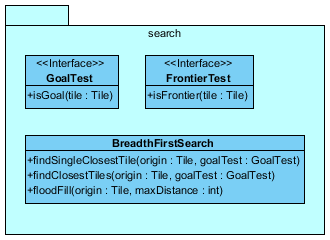
\includegraphics[width=0.7\textwidth]{91_bilder/BFS}
\caption{Breitensuche Klassendiagramm}
\label{fig:BFS}
\end{figure}

\begin{figure}[H]
\centering
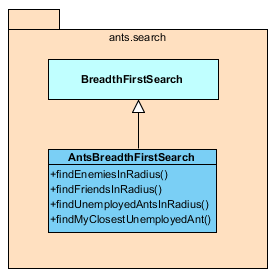
\includegraphics[width=0.5\textwidth]{91_bilder/BFSants}
\caption{Breitensuche Ants-spezifisch}
\label{fig:BFSants}
\end{figure}
Die Breitensuche (engl. breadth-first search (BFS)) war eine der Neuimplementierungen w�hrend der Bachelorarbeit. Man k�nnte die BFS auch f�r die Pfadsuche verwenden, dies w�re aber sehr ineffizient. Wir verwenden diese Suche vielmehr f�r die Umgebung einer Ameise oder eines H�gels zu analysieren. Sie wurde generisch implementierte, so dass sie vielseitig einsetzbar ist. So k�nnen zum Beispiel mittels 'GoalTest' je nach Anwendungsfall die Tiles beschrieben werden welche gesucht sind. Folgende Breitensuche findet die Ameise welche am n�chsten bei einem Food-Tile <r:20,c:16> ist. Sie wird initialisiert indem im Konstruktor die Spielkarte mitgegeben wird, welche durchforscht wird. Zus�tzlich gilt die Einschr�nkung das die Breitensuche nur 40 Tiles durchsuchen darf, was einem Radius von zirka 7 entspricht. Falls keine Ameise gefunden wird gibt der Algorithmus NULL zur�ck.

\begin{verbatim}
AntsBreadthFirstSearch bfs = new AntsBreadthFirstSearch(Ants.getWorld());
Tile food = new Tile(20,16);
Tile antClosestToFood = bfs.findSingleClosestTile(food, 40, new GoalTest() {
      @Override
      public boolean isGoal(Tile tile) {
          return isAntOnTile(tile);
      }
  });
\end{verbatim}

Es ist auch m�glich mehrere Tiles zur�ck zu bekommen. Dazu wird die Methode \textit{findClosestTiles(...)} aufgerufen.
\newline
\newline

Der gleiche Algorithmus kann aber auch alle passierbaren Tiles in einem gewissen Umkreis zur�ckgeben. Dies haben wir unter anderem beim Initialisieren der DefendHillMission verwendet. Wir berechnen beim Erstellen der Mission die passierbaren Tiles rundum den H�gel. Runde f�r Runde pr�fen wir diese Tiles auf gegnerische Ameisen um die entsprechenden Verteidigungsmassnahmen zu ergreifen. Der Parameter controlAreaRadius2 definiert den Radius des 'Radars' und kann je nach Profile unterschiedlich eingestellt werden.

\begin{verbatim}
public DefendHillMission(Tile myhill) {
    this.hill = myhill;
    BreadthFirstSearch bfs = new BreadthFirstSearch(Ants.getWorld());
    tilesAroundHill = bfs.floodFill(myhill, controlAreaRadius2);
}
\end{verbatim}

\subsection{Barrier}
\label{subsec:module.Suchalgorithmen.Breitensuche.Barrier}

Eine Erweiterung der Breitensuche erm�glicht uns eine Sperre in der Umgebung eines Ortes zu finden. Diese Verwenden wir in der DefendHillMission zum Verteidigen des eigenen H�gels. Es kann nur eine Sperre (engl. Barrier) gefunden werden wenn das Gel�nde dazu passt. Der Algorithmus verbirgt sich in der Methode \textit{getBarrier(...)}. Diese wird mit den Parametern tileToProtect: Ort f�r den eine Sperre berechnet werden soll, viewRadiusSquared: den Sicht Radius der Einheiten, den die Sperre soll weiter entfernt sein als der Sichtradius, damit die gegnerischen Einheiten nicht sehen was sich dahinter verbirgt. Der dritte Parameter maximumBarrierSize definiert wie breit die Sperre maximal sein darf.

\begin{verbatim}
public Barrier getBarrier(final Tile tileToProtect, int viewRadiusSquared, int maximumBarrierSize) {
	int amount = BFS for getting the amount of tiles in view radius around the location to defend.
	Barrier smallestBarrier = null;
	List<Tile> tiles = get (amount + 30) tiles around the location to defend.
	
	for(int i = amount;i<tiles.size(); i++){       
		Tile t = tiles.get(i);
		
		//vertical check
		if(!barrierVerticalInvalid.contains(t)){
			Barrier b = get vertical barrier on position of Tile t
			if(b is smaller than 5 Tiles && smaller than smallestBarrier){
				if(is barrier the only exit out of the location to defend){
						smallestBarrier = b;
				}else{
						barrierVerticalInvalid.add(b.getTiles());
				}    					      		
			}else{
				barrierVerticalInvalid.add(b.getTiles());
			}
		}
		
		//horizontal check
		if(!barrierHorizontalInvalid.contains(t)){
			Barrier b = get horiontal barrier on position of Tile t
			if(b is smaller than 5 Tiles && smaller than smallestBarrier){
				if(is barrier the only exit out of the location to defend){
						smallestBarrier = b;
				}else{
						barrierHorizontalInvalid.add(b.getTiles());
				}    					      		
			}else{
				barrierHorizontalInvalid.add(b.getTiles());
			}
		}	
	}
}
\end{verbatim}

Dank dem Abspeichern der ung�ltigen Tiles aller zu breiten Sperren in \textit{barrierHorizontalInvalid} und \textit{barrierVerticalInvalid} konnte der Algorithmus markant schneller gemacht werden. F�r diese Tiles muss nicht nochmals eine Sperre berechnet werden. Auch die if-Abfrage \textit{barrier is the only exit out of the location to defend} muss nicht mehr so oft aufgerufen werden. Hinter dieser Abfrage steht n�mlich wiederum ein Test mit der Breitensuche. Dieser ist viel teurer als das zwischenspeichern der Tiles aus welchen keine g�ltige Sperre gemacht werden konnte.